\begin{figure}[!ht]
\begin{center}
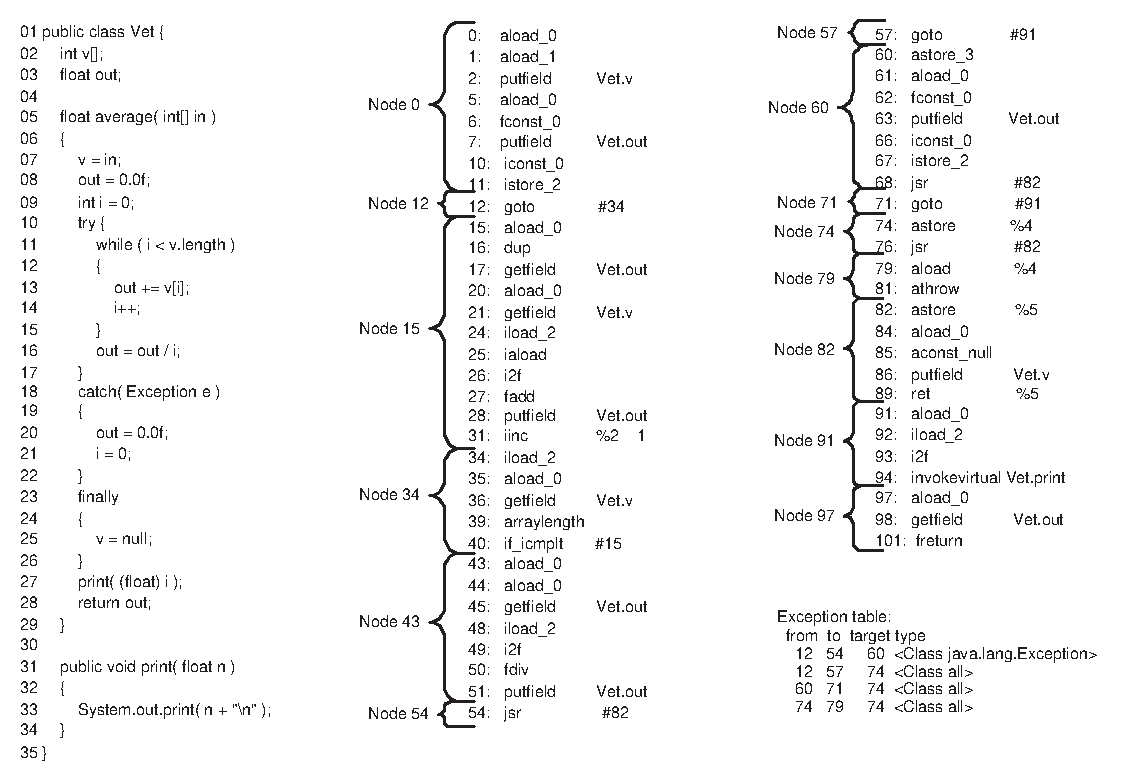
\includegraphics[scale=0.70]{fig/fig-bytecode.eps}
\caption{A simple Java program, its bytecode instructions and the
basic blocks.}\label{fig-bytecode}
\end{center}
\end{figure}


\begin{comment}
\scriptsize
\begin{tabular}{lll}
\begin{minipage}{0.3\textwidth}
\begin{verbatim}

01 public class Vet {
02     int v[];
03     float out;
04
05     float average( int[] in )
06     {
07         v = in;
08         out = 0.0f;
09         int i = 0;
10         try {
11             while ( i < v.length )
12             {
13                 out += v[i];
14                 i++;
15             }
16             out = out / i;
17         }
18         catch( Exception e )
19         {
20             out = 0.0f;
21             i = 0;
22         }
23         finally
24         {
25             v = null;
26         }
27         print( (float) i );
28         return out;
29     }
30
31     public void print( float n )
32     {
33         System.out.print( n + "\n" );
34     }
35 }

\end{verbatim}
\end{minipage}
&
\begin{minipage}{0.3\textwidth}
\begin{verbatim}
0:    aload_0
1:    aload_1
2:    putfield      Vet.v
5:    aload_0
6:    fconst_0
7:    putfield      Vet.out
10:   iconst_0
11:   istore_2
12:   goto          #34
15:   aload_0
16:   dup
17:   getfield      Vet.out
20:   aload_0
21:   getfield      Vet.v
24:   iload_2
25:   iaload
26:   i2f
27:   fadd
28:   putfield      Vet.out
31:   iinc          %2    1
34:   iload_2
35:   aload_0
36:   getfield      Vet.v
39:   arraylength
40:   if_icmplt     #15
43:   aload_0
44:   aload_0
45:   getfield      Vet.out
48:   iload_2
49:   i2f
50:   fdiv
51:   putfield      Vet.out
54:   jsr           #82
57:   goto          #91
60:   astore_3
61:   aload_0
62:   fconst_0
63:   putfield      Vet.out
66:   iconst_0
67:   istore_2
68:   jsr           #82
71:   goto          #91
74:   astore        %4
76:   jsr           #82
79:   aload         %4
81:   athrow
82:   astore        %5
84:   aload_0
85:   aconst_null
86:   putfield      Vet.v
89:   ret           %5
91:   aload_0
92:   iload_2
93:   i2f
94:   invokevirtual Vet.print
97:   aload_0
98:   getfield      Vet.out
101:  freturn
\end{verbatim}
\end{minipage}
\end{tabular}
\end{center}
\caption{A simple Java program, its bytecode instructions and the basic blocks.}\label{fig-bytecode}
\end{figure}
\end{comment}
